\documentclass[10pt,twocolumn]{article}
\usepackage[margin=0.62in]{geometry}
\usepackage{graphicx}
\usepackage{booktabs}
\usepackage{array}
\usepackage{caption}
\usepackage[hidelinks]{hyperref}

\setlength{\parindent}{0pt}
\setlength{\parskip}{3pt}
\setlength{\columnsep}{0.22in}
\captionsetup{font=footnotesize, labelfont=bf}
\makeatletter
\renewcommand\section{\@startsection {section}{1}{\z@}%
  {-0.8ex \@plus -0.2ex \@minus -.2ex}%
  {0.35ex \@plus.1ex}%
  {\normalfont\large\bfseries}}
\makeatother

\newcommand{\fcorr}{F_{\mathrm{corr}}}

\title{\vspace{-1.2cm}\textbf{Structure and Function in a MICrONS Visual-Cortex Network}}
\author{}
\date{\vspace{-1.0cm}}

\begin{document}
\maketitle
\thispagestyle{empty}
\pagestyle{empty}

\section{Introduction}
How strongly does synaptic wiring predict neural activity? This is a central question in functional connectomics: structural graphs describe possible communication pathways, while functional graphs describe co-variation in measured responses. In visual cortex, previous work supports ``like-to-like'' wiring, where neurons with similar stimulus responses are more likely to be connected \cite{ko2011,cossell2015,ding2025}. The MICrONS dataset makes this question accessible at larger scale by co-registering calcium-imaging responses with electron-microscopy connectivity across mouse visual areas \cite{microns2025}. 

This project relates directly to course topics on graph representation and network comparison. The structural network is sparse, directed, and weighted by synaptic size/count; the functional network is dense, symmetric, and signed because it is built from response correlations. The analysis therefore asks not only whether individual connected pairs are more correlated, but also whether the two networks share broader topology such as degree, strength, hubness, and clustering.

\section{Research Questions}
The primary question was: are directly connected neuron pairs more functionally correlated than unconnected pairs? Secondary questions asked whether the effect is graded by synapse strength, enhanced by reciprocity, robust to distance, area, layer, cell type, and orientation controls, visible in a same-scan validation cohort, and reflected in network-level topology.

\section{Methodology}
The main analysis used 906 functionally matched excitatory neurons from the MICrONS visual-cortex data. Functional similarity was defined as pairwise signal correlation, $\fcorr$, across shared oracle-response vectors. Structural connectivity was loaded from the directed structural edge table, using the convention that $C_{ij}$ is a synaptic edge from presynaptic neuron $i$ to postsynaptic neuron $j$. The pair-level table contained all 409,965 unordered neuron pairs, with labels for unconnected, unidirectional, and bidirectional connectivity; summed synapse size; soma-soma distance; area, layer, and cell-type composition; and orientation-similarity measures where available.

The pipeline proceeded in stages. First, connected and unconnected pairs were compared using mean differences, bootstrap confidence intervals, Mann-Whitney tests, and neuron-identity permutation nulls. Second, connected pairs were tested for graded structure-function alignment using Spearman correlation between summed synapse size and $\fcorr$. Third, bidirectional pairs were compared with unidirectional and unconnected pairs. Fourth, the main pair-level result was stress-tested using distance matching, within-distance-bin contrasts, logistic regression with distance terms, stratification by composition, joint logistic models, and a well-tuned orientation subset. Finally, topology was evaluated by comparing structural degree/strength to node-level mean functional coupling, with partial Spearman controls and matched-density thresholded functional graphs.

A smaller same-scan validation used 93 V1/L4 neurons from scan 9.3. This cohort allowed trace-correlation, signal-correlation, and noise-correlation versions of the connected-versus-unconnected comparison, providing a measurement-regime check on the larger 906-neuron signal-correlation analysis.

\section{Results}
The main pair-level result was positive and robust. In the 906-neuron cohort, connected pairs had higher signal correlation than unconnected pairs: $\Delta\bar{\fcorr}=0.0334$ with 95\% CI $[0.0307,0.0360]$. A neuron-identity permutation null placed the observed effect about 20.6 standard deviations above the null mean, so the result was not explained by a random reassignment of neuron identities to the fixed structural graph. The absolute effect was modest, but the distributional shift was consistent.

Structural weight added a weak graded component. Among connected pairs, summed synapse size correlated positively with $\fcorr$ (Spearman $\rho=0.0686$, 95\% CI $[0.0501,0.0864]$). Thus edge weight carried additional information beyond the binary connected label, but explained only a small fraction of pairwise response similarity. Reciprocity was less convincing: bidirectional pairs had the highest mean $\fcorr$ and unconnected pairs the lowest, but the bidirectional-minus-unidirectional contrast was not detected under the permutation test ($p=0.090$).

Controls narrowed but did not remove the pair-level claim. Distance was a major confound: connection probability and mean $\fcorr$ covaried strongly across distance bins. After matching every connected pair to a closest-distance unconnected control, the connected-pair effect shrank from about 0.033 to 0.0186, but remained positive. The effect also remained positive within distance bins and in a logistic model controlling for distance and distance squared. Composition controls gave the same qualitative answer: $\fcorr$ remained a positive predictor in a joint model with distance, same-area, same-layer, and same-cell-type indicators (standardized $\beta=0.130$, 95\% CI $[0.112,0.148]$). In the well-tuned subset, orientation similarity was also higher for connected pairs, but $\fcorr$ remained the stronger predictor when orientation similarity and distance were modeled jointly.

The validation and scope checks supported the main result without making it universal. In the 93-neuron V1/L4 same-scan cohort, connected pairs were more correlated by trace correlation ($\Delta=0.0258$, 95\% CI $[0.0182,0.0342]$), signal correlation ($\Delta=0.0529$), and noise correlation ($\Delta=0.0466$). Within the 906-neuron cohort, the effect was clearest in V1, weaker in RL, unresolved in AL, and positive across areas; the non-V1 within-area tests were underpowered because the cohort is strongly imbalanced.

Network topology showed a more limited result. The primary node-level hub analysis found a weak partial Spearman relationship between total structural strength and mean signed functional coupling after distance and area controls ($\rho=0.110$, about 1.2\% rank-variance approximation). However, this signal weakened under stricter controls and was not reproduced by absolute functional coupling. In matched-density thresholded functional graphs, structural degree and functional degree were nearly uncoupled ($\rho=0.0082$, $p=0.805$ at matched density), even though functional clustering was higher than structural clustering.

\section{Discussion}
The research question is answered positively at the pair level but negatively, or at least inconclusively, at the topology level. Direct synaptic connectivity predicts a higher expected functional similarity, and this remains true after the most important controls available in the notebook. The effect should not be read as deterministic: most connected pairs are still only modestly correlated, and structural information explains a small part of functional variation. The best interpretation is enrichment, not one-to-one prediction.

The controls are important because nearby neurons, same-area neurons, and similarly tuned neurons are all more likely to be both connected and functionally similar. Distance matching and composition models show that these factors explain part of the raw effect, but not all of it. The orientation analysis further suggests that signal correlation is not merely a proxy for one tuning axis. This is consistent with prior like-to-like wiring results, while preserving a narrower conclusion appropriate for this analysis.

The main limitation is dependence and incompleteness. Pair rows are not independent because each neuron appears in many pairs; permutation tests help but do not fully solve all hierarchical dependence. The structural graph is also a proofread/matched subset rather than a complete connectome, and the functional graph depends on the chosen response metric. The topology analysis is especially sensitive to definitions because sparse directed synapses and dense symmetric correlations are mathematically different objects. Future work should use hierarchical or mixed-effects models, axon-dendrite opportunity controls, richer tuning decompositions, and repeated animals or scans. The strongest current conclusion is therefore specific: structural connectivity carries a robust but modest pair-level functional signal, while broader structural-functional topology matching was not detected.

\clearpage
\onecolumn

\section*{Figures and Tables}
\begin{figure}[h]
  \centering
  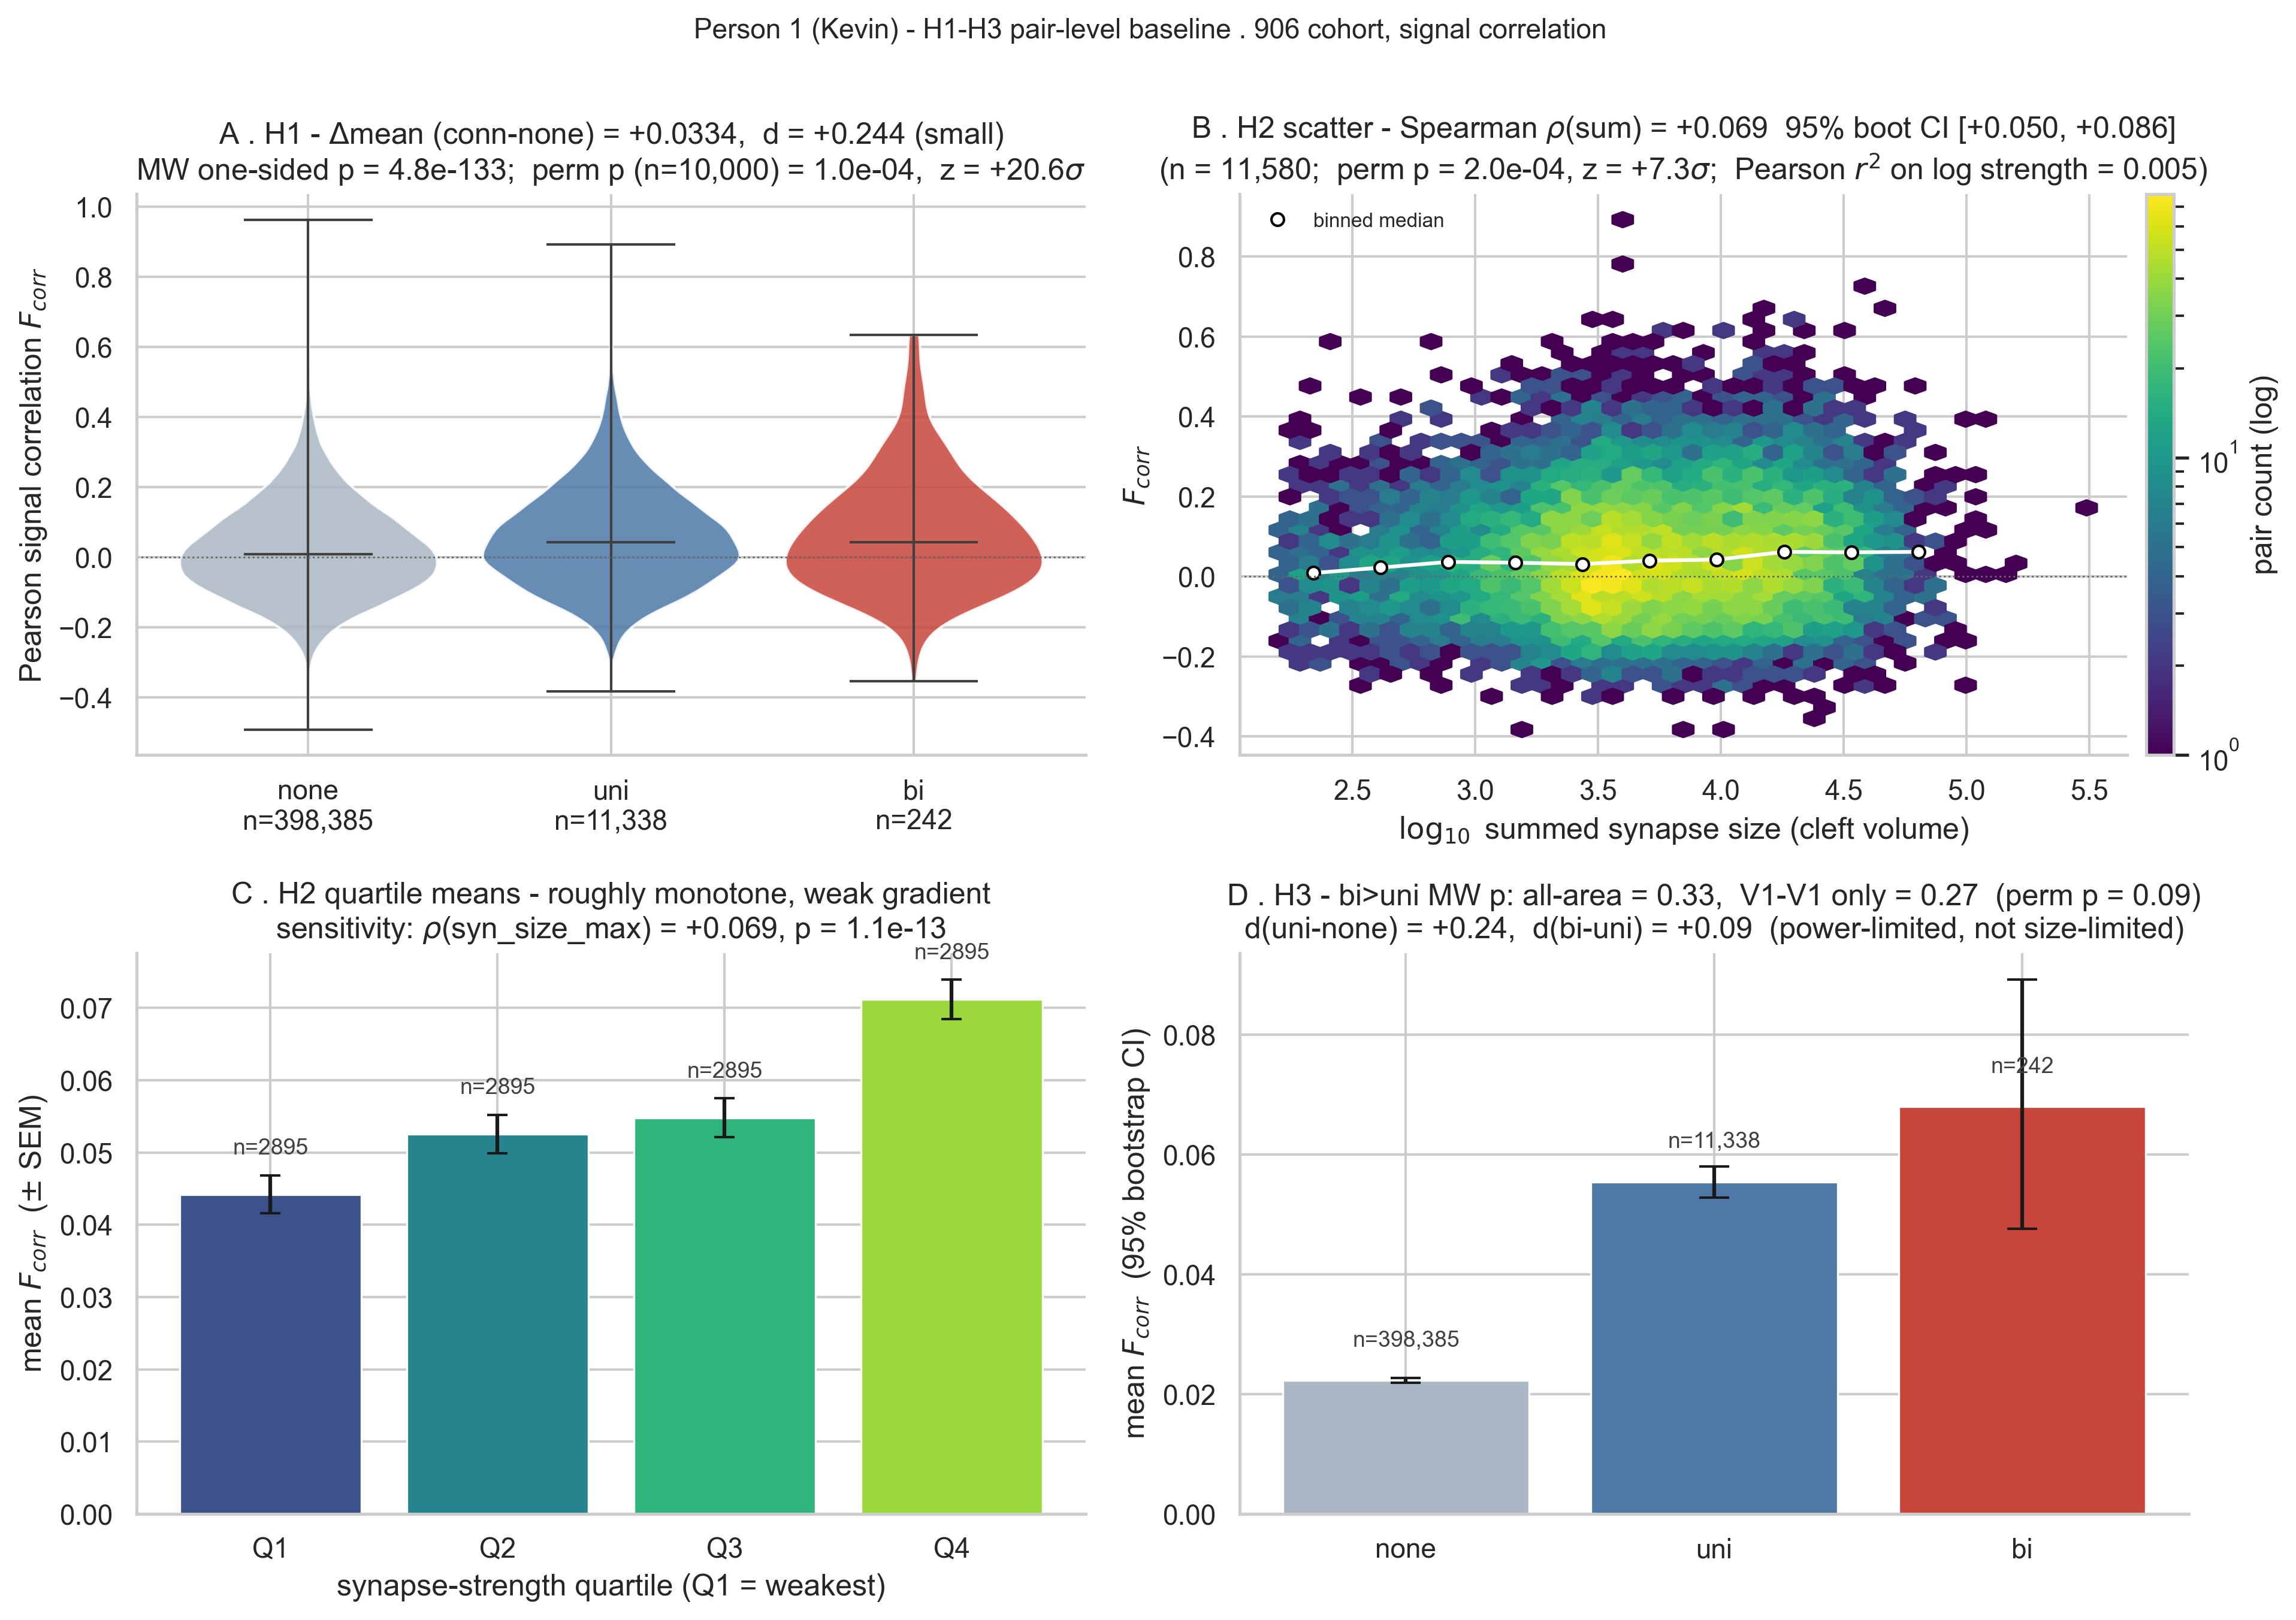
\includegraphics[width=0.95\textwidth]{outputs/figures/person1_h1_h3_pair_baseline.png}
  \caption{Baseline pair-level results for connected, unidirectional, bidirectional, and unconnected neuron pairs in the 906-neuron cohort.}
  \label{fig:h1h3}
\end{figure}

\begin{figure}[h]
  \centering
  \begin{minipage}{0.48\textwidth}
    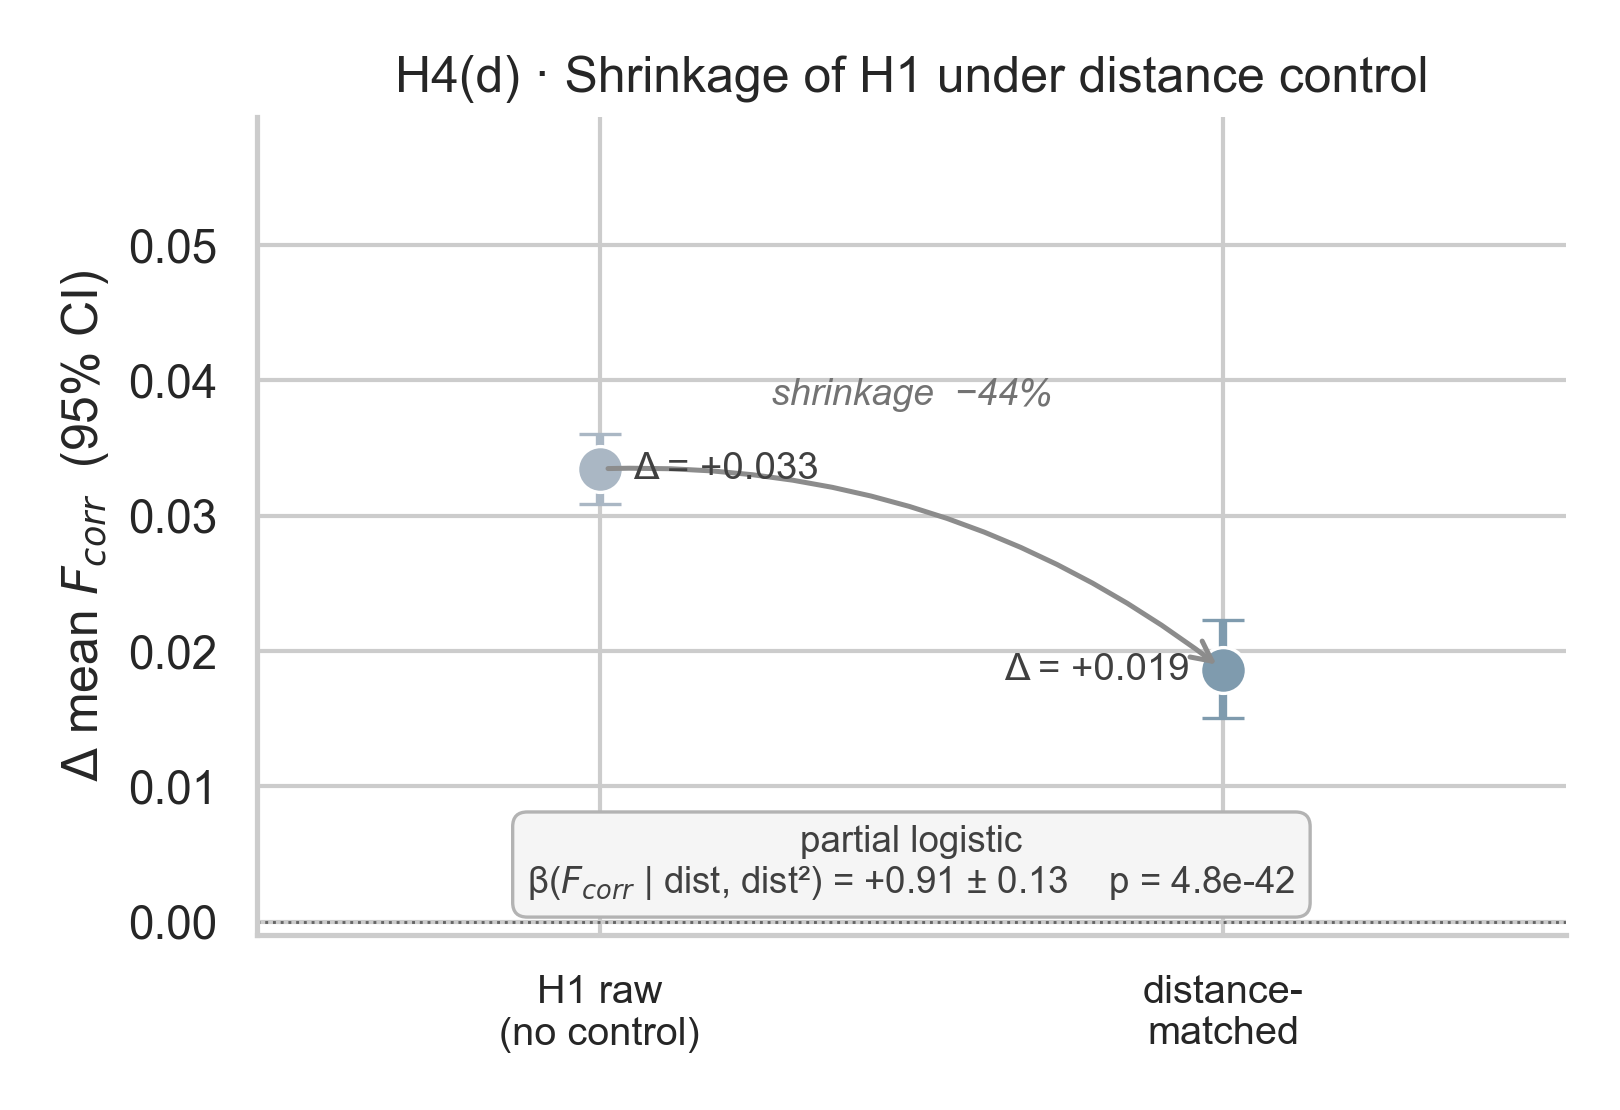
\includegraphics[width=\linewidth]{outputs/figures/H4d_shrinkage.png}
  \end{minipage}
  \hfill
  \begin{minipage}{0.48\textwidth}
    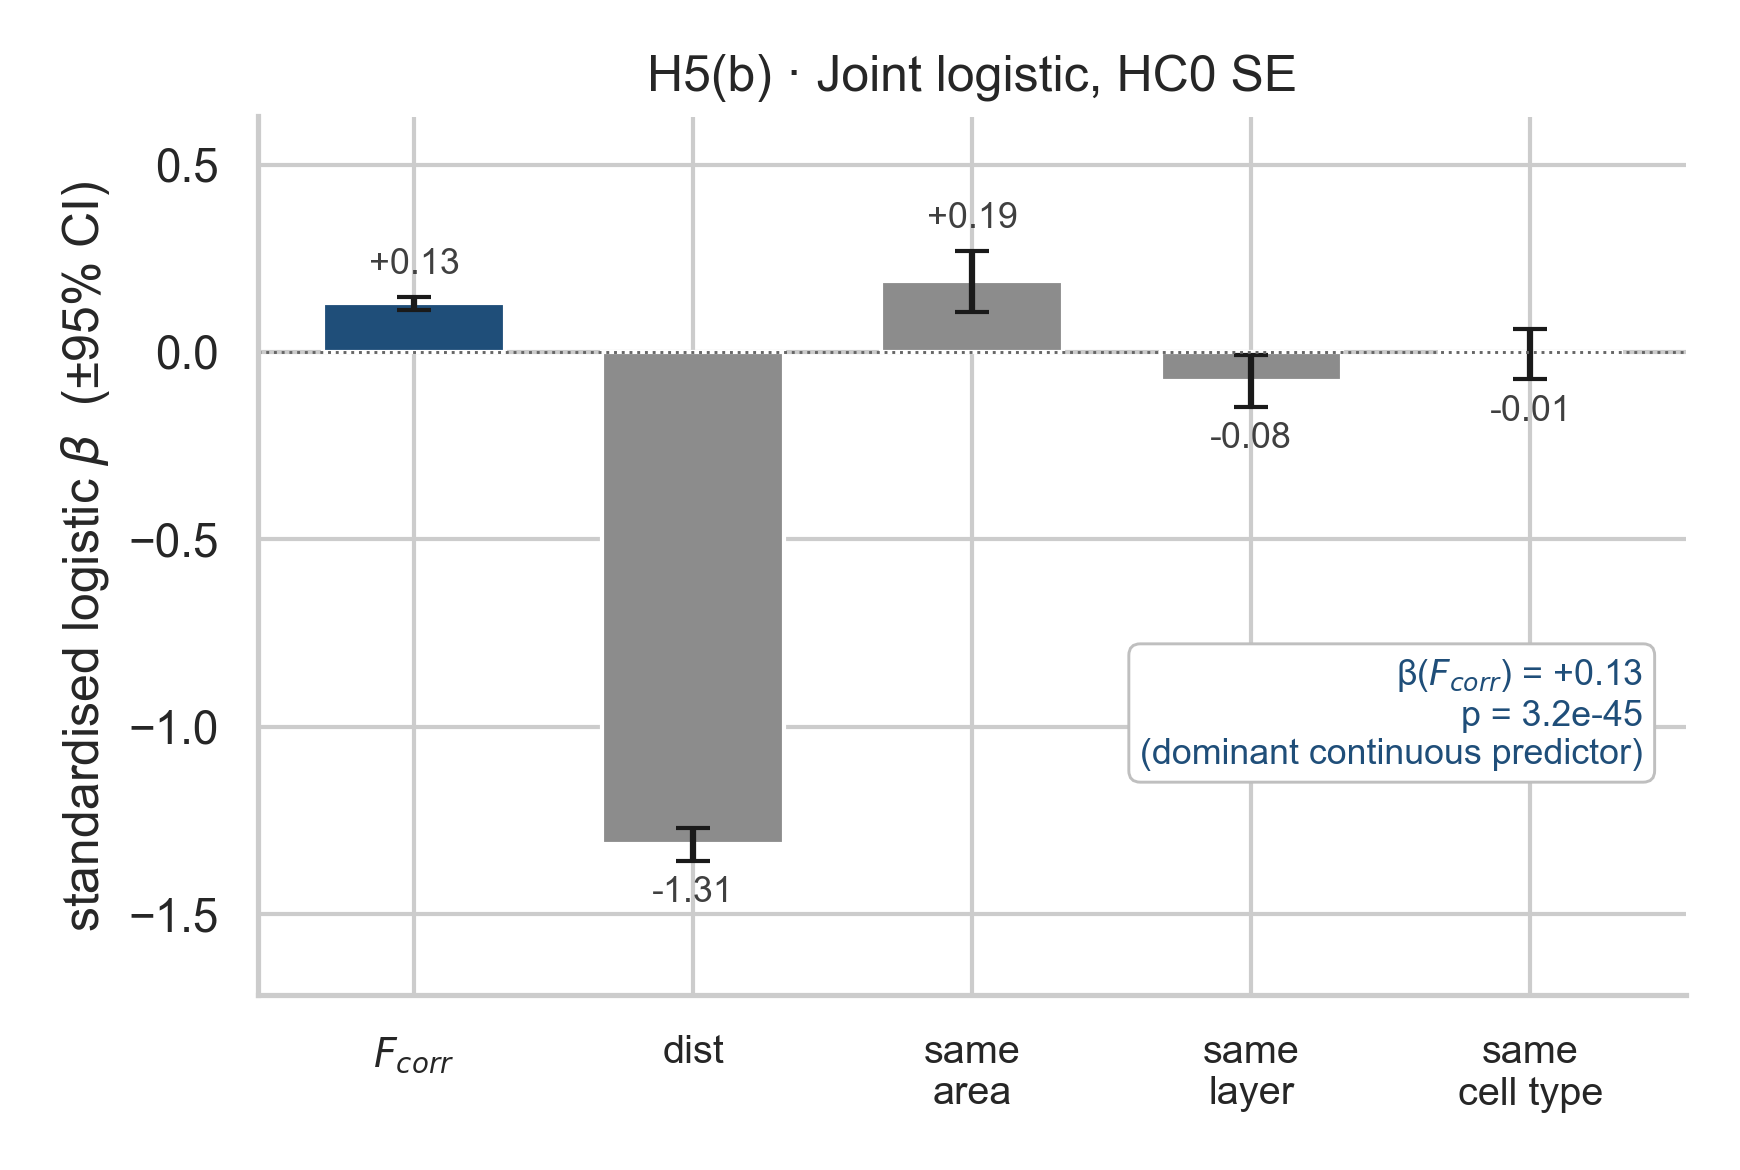
\includegraphics[width=\linewidth]{outputs/figures/H5b_joint_logistic.png}
  \end{minipage}
  \caption{Main controls. Left: the connected-pair effect shrinks but remains positive after distance matching. Right: standardized joint-model coefficients with composition controls.}
  \label{fig:controls}
\end{figure}

\begin{figure}[h]
  \centering
  \begin{minipage}{0.48\textwidth}
    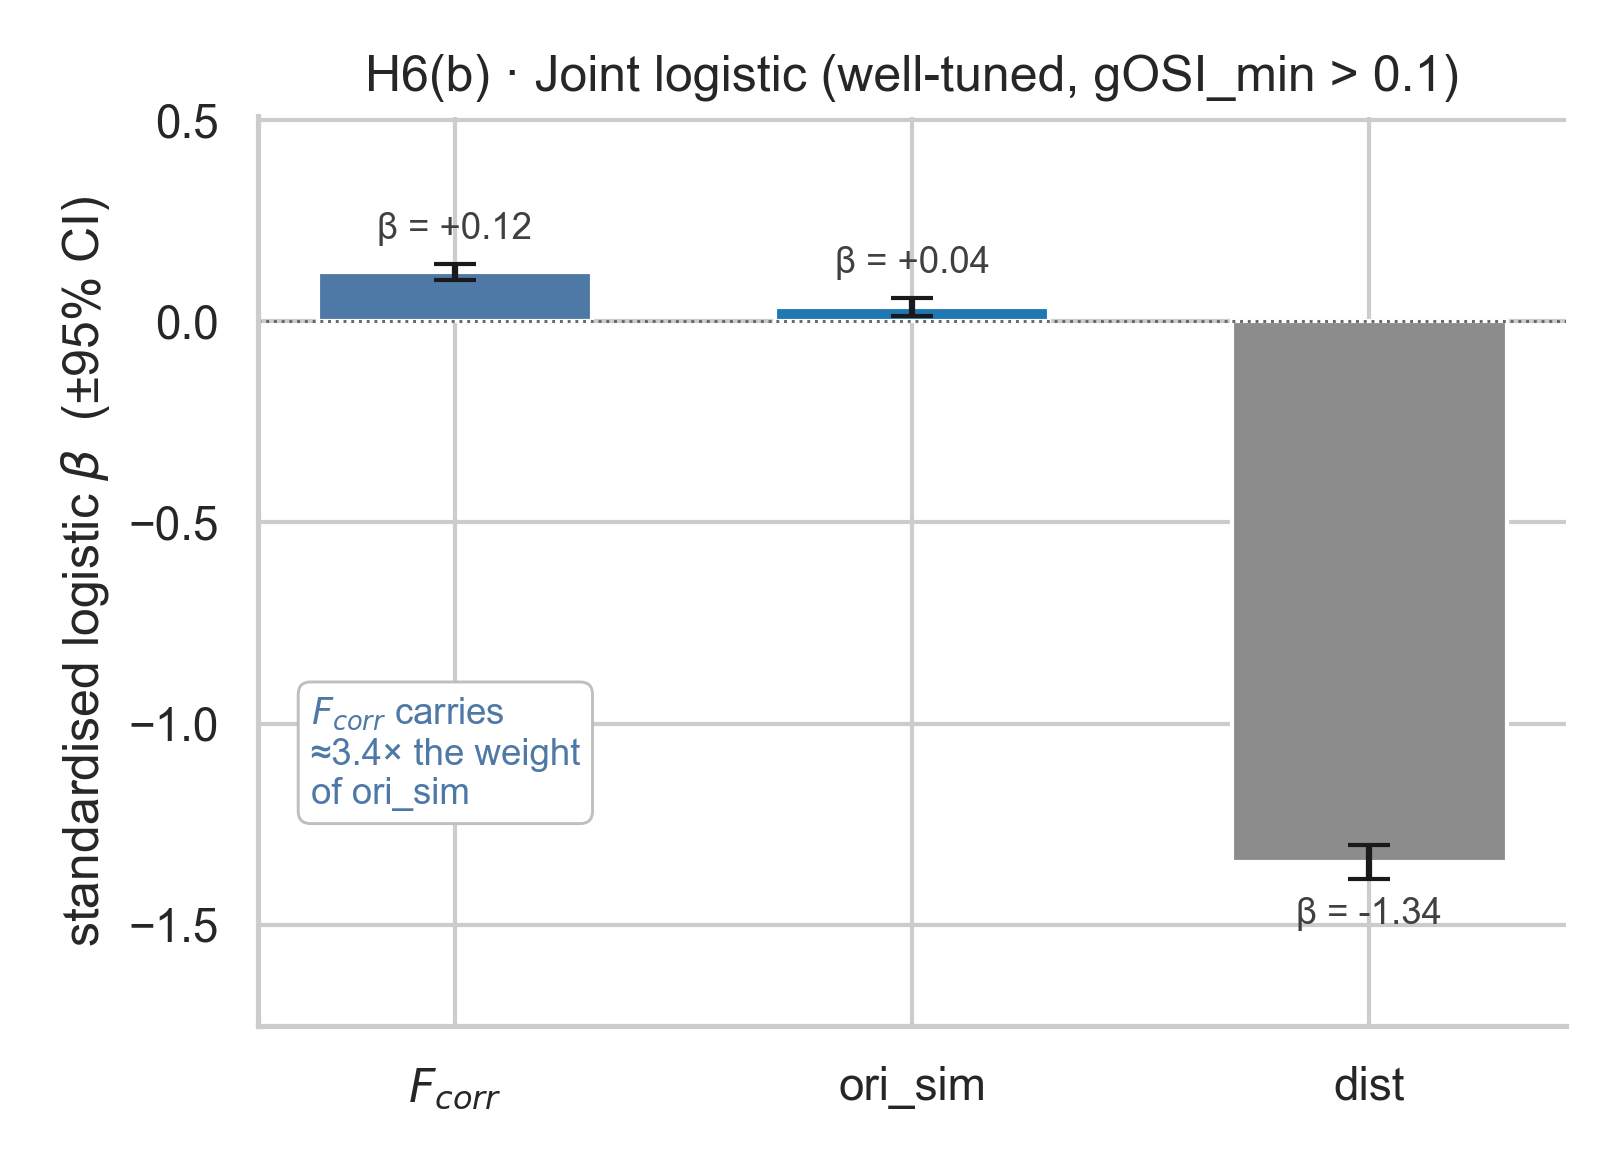
\includegraphics[width=\linewidth]{outputs/figures/H6b_joint_logistic.png}
  \end{minipage}
  \hfill
  \begin{minipage}{0.48\textwidth}
    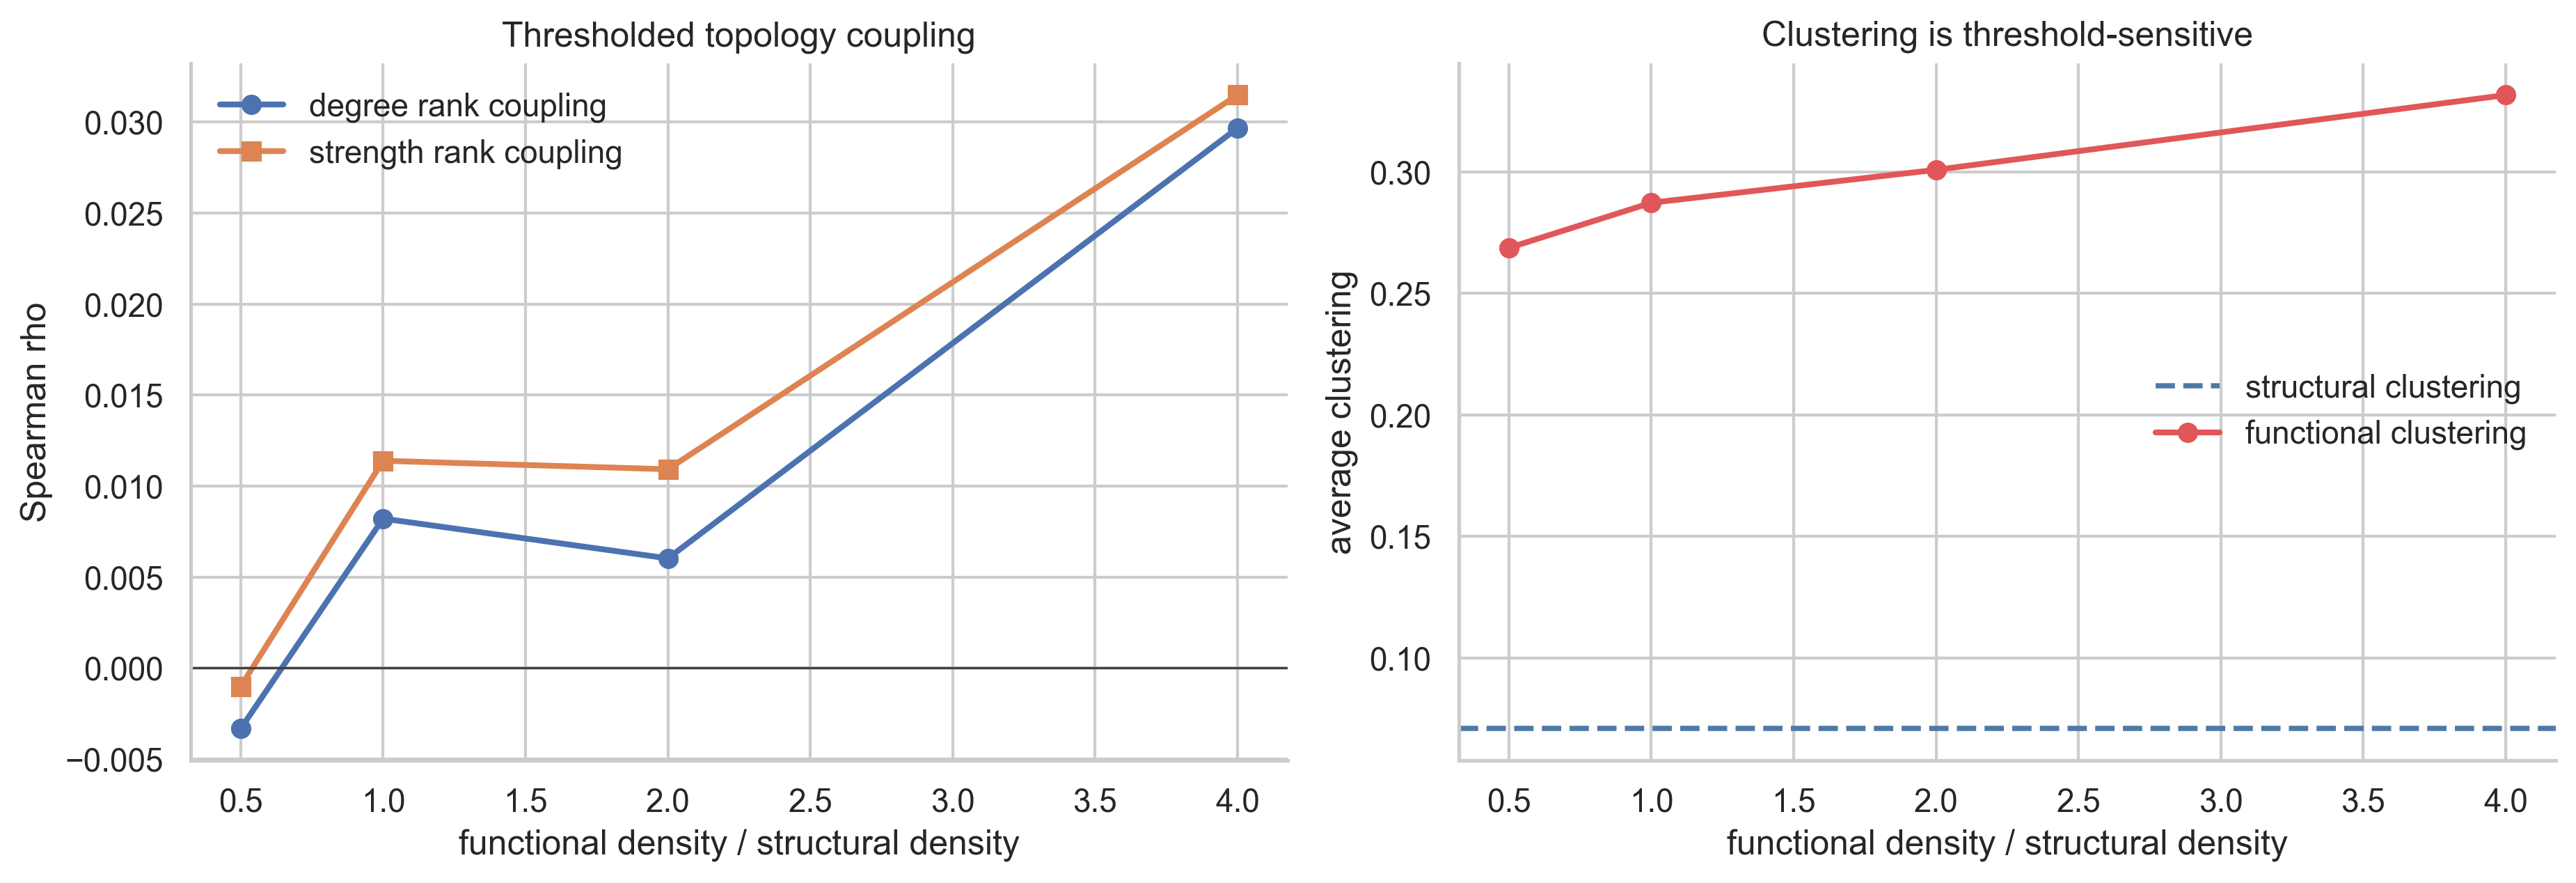
\includegraphics[width=\linewidth]{outputs/figures/h7_topology_sensitivity.png}
  \end{minipage}
  \caption{Orientation and topology checks. Signal correlation remains stronger than orientation similarity in the well-tuned subset, while thresholded graph topology shows near-zero structural-functional degree or strength coupling.}
  \label{fig:h6h7}
\end{figure}

\begin{figure}[h]
  \centering
  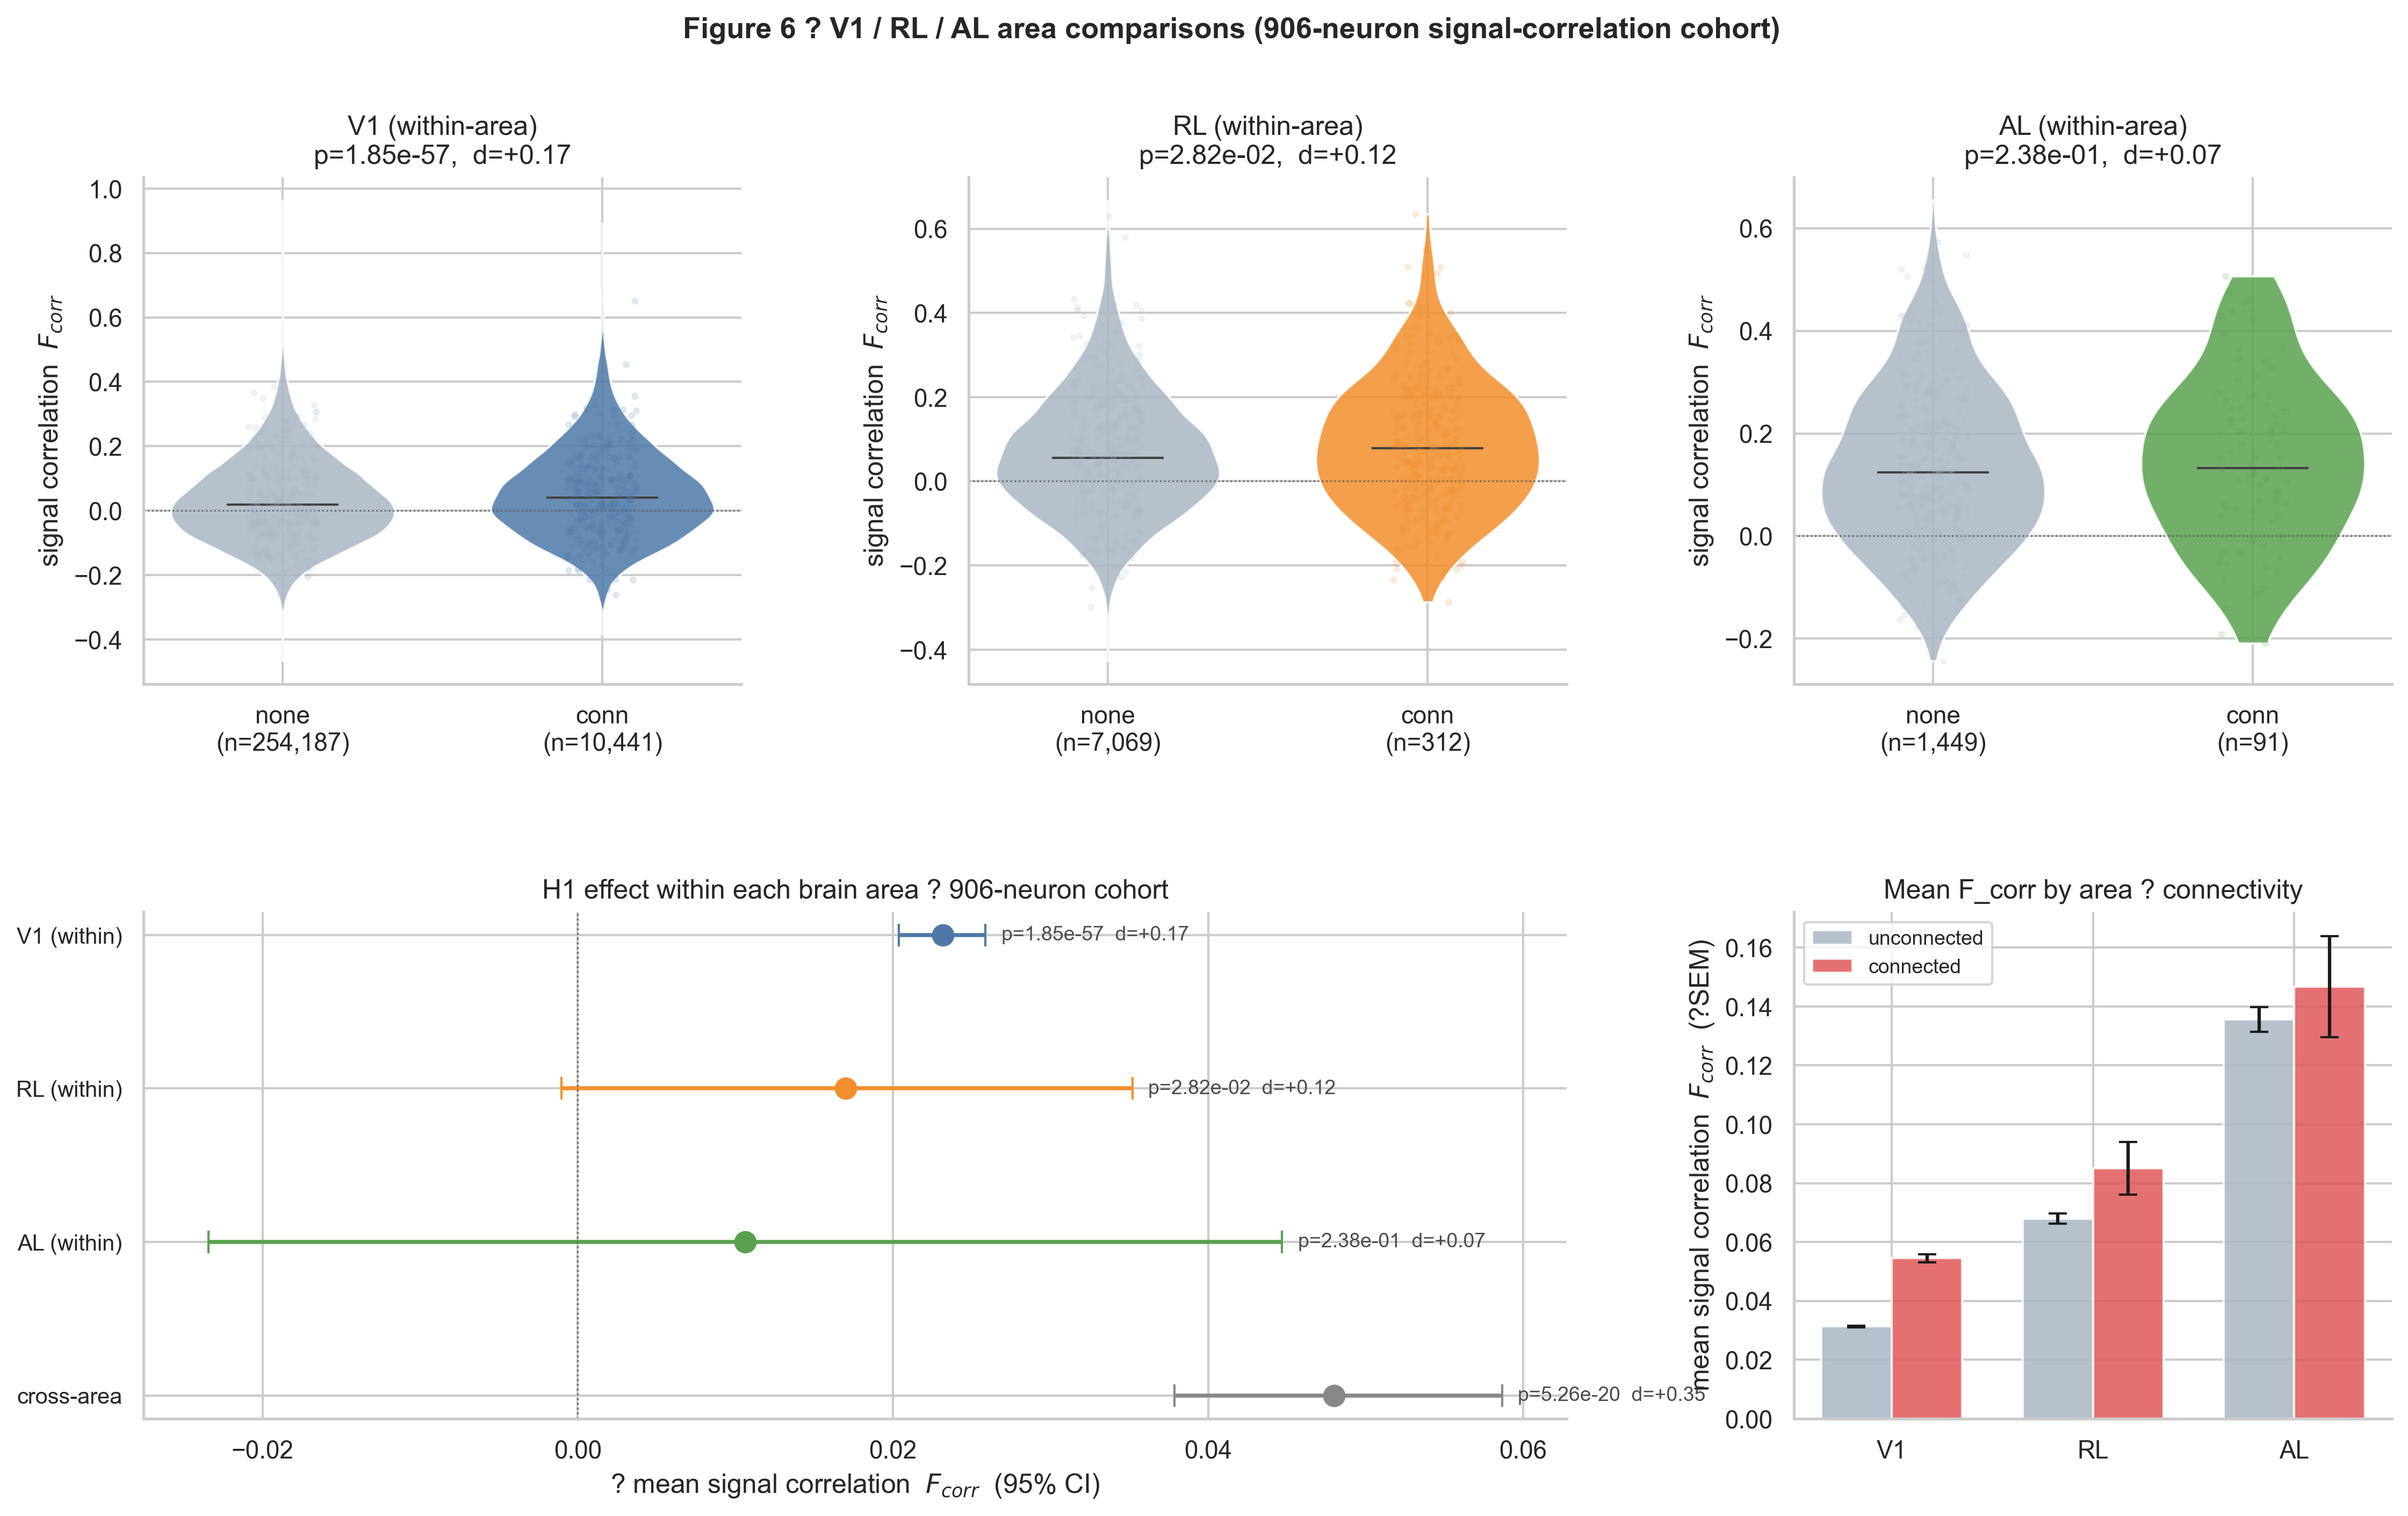
\includegraphics[width=0.95\textwidth]{outputs/figures/person4_scan93_area_checks.png}
  \caption{Same-scan 93-neuron validation and exploratory V1/RL/AL area-scope checks.}
  \label{fig:validation}
\end{figure}

\begin{table}[h]
\centering
\small
\caption{Compact summary of the notebook's main quantitative results.}
\begin{tabular}{>{\raggedright\arraybackslash}p{0.17\textwidth}
                >{\raggedright\arraybackslash}p{0.36\textwidth}
                >{\raggedright\arraybackslash}p{0.17\textwidth}
                >{\raggedright\arraybackslash}p{0.20\textwidth}}
\toprule
Analysis & Question & Effect & Interpretation \\
\midrule
H1 & Connected vs. unconnected pairs & $\Delta\bar{\fcorr}=0.0334$ & Supported; robust pair-level enrichment. \\
H2 & Synapse strength gradient & $\rho=0.0686$ & Supported but weak. \\
H3 & Bidirectional vs. unidirectional & $\Delta=0.0126$, perm. $p=0.090$ & Reciprocity premium not detected. \\
H4 & Distance control & $\Delta=0.0186$ after matching & Effect shrinks but remains positive. \\
H5 & Composition controls & std. $\beta_{\fcorr}=0.130$ & Positive after distance, area, layer, cell type. \\
H6 & Orientation control & std. $\beta_{\fcorr}=0.122$ & Not just orientation similarity. \\
H7 & Hub/topology alignment & partial $\rho=0.110$; matched-degree $\rho=0.008$ & Weak signed hub signal; topology matching not detected. \\
Validation & 93-neuron V1/L4 same-scan & trace $\Delta=0.0258$ & H1 replicated across trace, signal, and noise views. \\
\bottomrule
\end{tabular}
\end{table}

\begin{thebibliography}{9}
\bibitem{ko2011}
Ko, H., Hofer, S. B., Pichler, B., Buchanan, K. A., Sjostrom, P. J., and Mrsic-Flogel, T. D. Functional specificity of local synaptic connections in neocortical networks. \textit{Nature} 473, 87--91 (2011). \url{https://doi.org/10.1038/nature09880}.

\bibitem{cossell2015}
Cossell, L., Iacaruso, M. F., Muir, D. R. \textit{et al.} Functional organization of excitatory synaptic strength in primary visual cortex. \textit{Nature} 518, 399--403 (2015). \url{https://doi.org/10.1038/nature14182}.

\bibitem{microns2025}
The MICrONS Consortium. Functional connectomics spanning multiple areas of mouse visual cortex. \textit{Nature} 640, 435--447 (2025). \url{https://doi.org/10.1038/s41586-025-08790-w}.

\bibitem{ding2025}
Ding, Z., Fahey, P. G., Papadopoulos, S. \textit{et al.} Functional connectomics reveals general wiring rule in mouse visual cortex. \textit{Nature} 640, 459--469 (2025). \url{https://doi.org/10.1038/s41586-025-08840-3}.
\end{thebibliography}

\end{document}
